\documentclass[10pt,letterpaper,oneside]{article}
\usepackage[top=.5in, bottom=.5in, left=.5in, right=.5in]{geometry}
\usepackage{nopageno} %Supresses page number at bottom
\usepackage{graphicx}
\usepackage{parskip}
\usepackage[compact]{titlesec}

\begin{document}

%Left margin, above skip, below skip
\titlespacing{\section}{0pt}{*4}{*0}
\titlespacing{\subsection}{0pt}{*1}{*0}
\titlespacing{\subsubsection}{0pt}{*1}{*0}

\centering
\begin{Huge}
\textsc{Team: The Saucy Winches}\\[.25cm]
\end{Huge}
\begin{Large}
John Anthony Dougherty and Ben Yarmis
\end{Large}

\hrulefill

\centering
\subsection*{Design}

\raggedright
The goal of this design project was to create a vehicle capable of winching itself along with a two pound weight up a forty-five degree slope and subsequently ``parking'' in the designated zone. When parked, the motor must be turned off, the vehicle must not roll backward, and the timing mechanism controlling engine cut-off must be entirely mechanical. To accomplish these objectives, a design was settled on consisting of a large diameter front wheel to conquer the initial forty-five degree turn and two rear marble casters made of plastic to minimize friction while providing stability. A worm gear transmission was used for the timing mechanism, which would reduce the rotational velocity enough for a cam to rotate about three-quarters of a revolution to physically hit the cut-off switch. The load is carried underneath the base plate to keep the vehicle's center of gravity as close to the ground as possible to avoid tipping.

\centering
\subsection*{Analysis}

\raggedright
The largest force acting on the spool shaft was determined to be the force due to the tension in the line having a magnitude of 3.48 lbf. The largest bending moment in the shaft occurs at the location of the spool and has a magnitude of 2 lbf-in, leading to a maximum bending stress of 1300 psi. When combined with the torsional stress in the shaft, the maximum normal stress in the shaft was determined to be 2093 psi, which is well below the yield strength of aluminum. The maximum deflection of the spool shaft was calculated to be 0.00145 inches, which is not enough to significantly affect gear alignment.

\centering
\subsection*{Cost}

\raggedright
The following parts were purchased: two spur gears for the power transmission, a worm gear with mating worm for the timing mechanism, and a ratchet and pawl for the braking system. The total cost of these components is \$27.08, which is well within the allowed budget of \$50.

\centering
\subsection*{Performance}

\raggedright
In competition, the vehicle performed very well, stopping inside the parking zone during both trials and scaling the ramp in the shortest amount of time among the non-disqualified vehicles. During the first run, when the vehicle abruptly came to a stop in the parking zone, the washer securing the line to the top of the ramp slid off the hook due to sudden slack in the line; however, this issue was not due to a flaw in the vehicle design and was easily resolved during the second run by better securing the washer. To improve the design, the weight would be better placed to keep the center of gravity in the middle of the vehicle, ensuring a straighter trajectory up the slope. Another improvement would be to fabricate a fairleader to keep the fishing line in the slit of the front wheel as it was initially designed. If the vehicle was going to be designed and manufactured again, the speed could be improved by reducing the weight and slightly reducing the gear ratio, leading to a lower torque output but higher rotational speed.

\centering
\subsection*{Conclusion}

\raggedright
In conclusion, the car worked as intended. It was able to winch itself up the ramp, stop in the designated parking zone, and hold itself there. Both the marble casters and plastic front wheel functioned well, as well as the timing and braking mechanisms. Neither deflections nor stresses were an issue in any of the shafts. Fabrication was completed several days before the due date and the car was under-budget.

\begin{figure}[b]
\centering
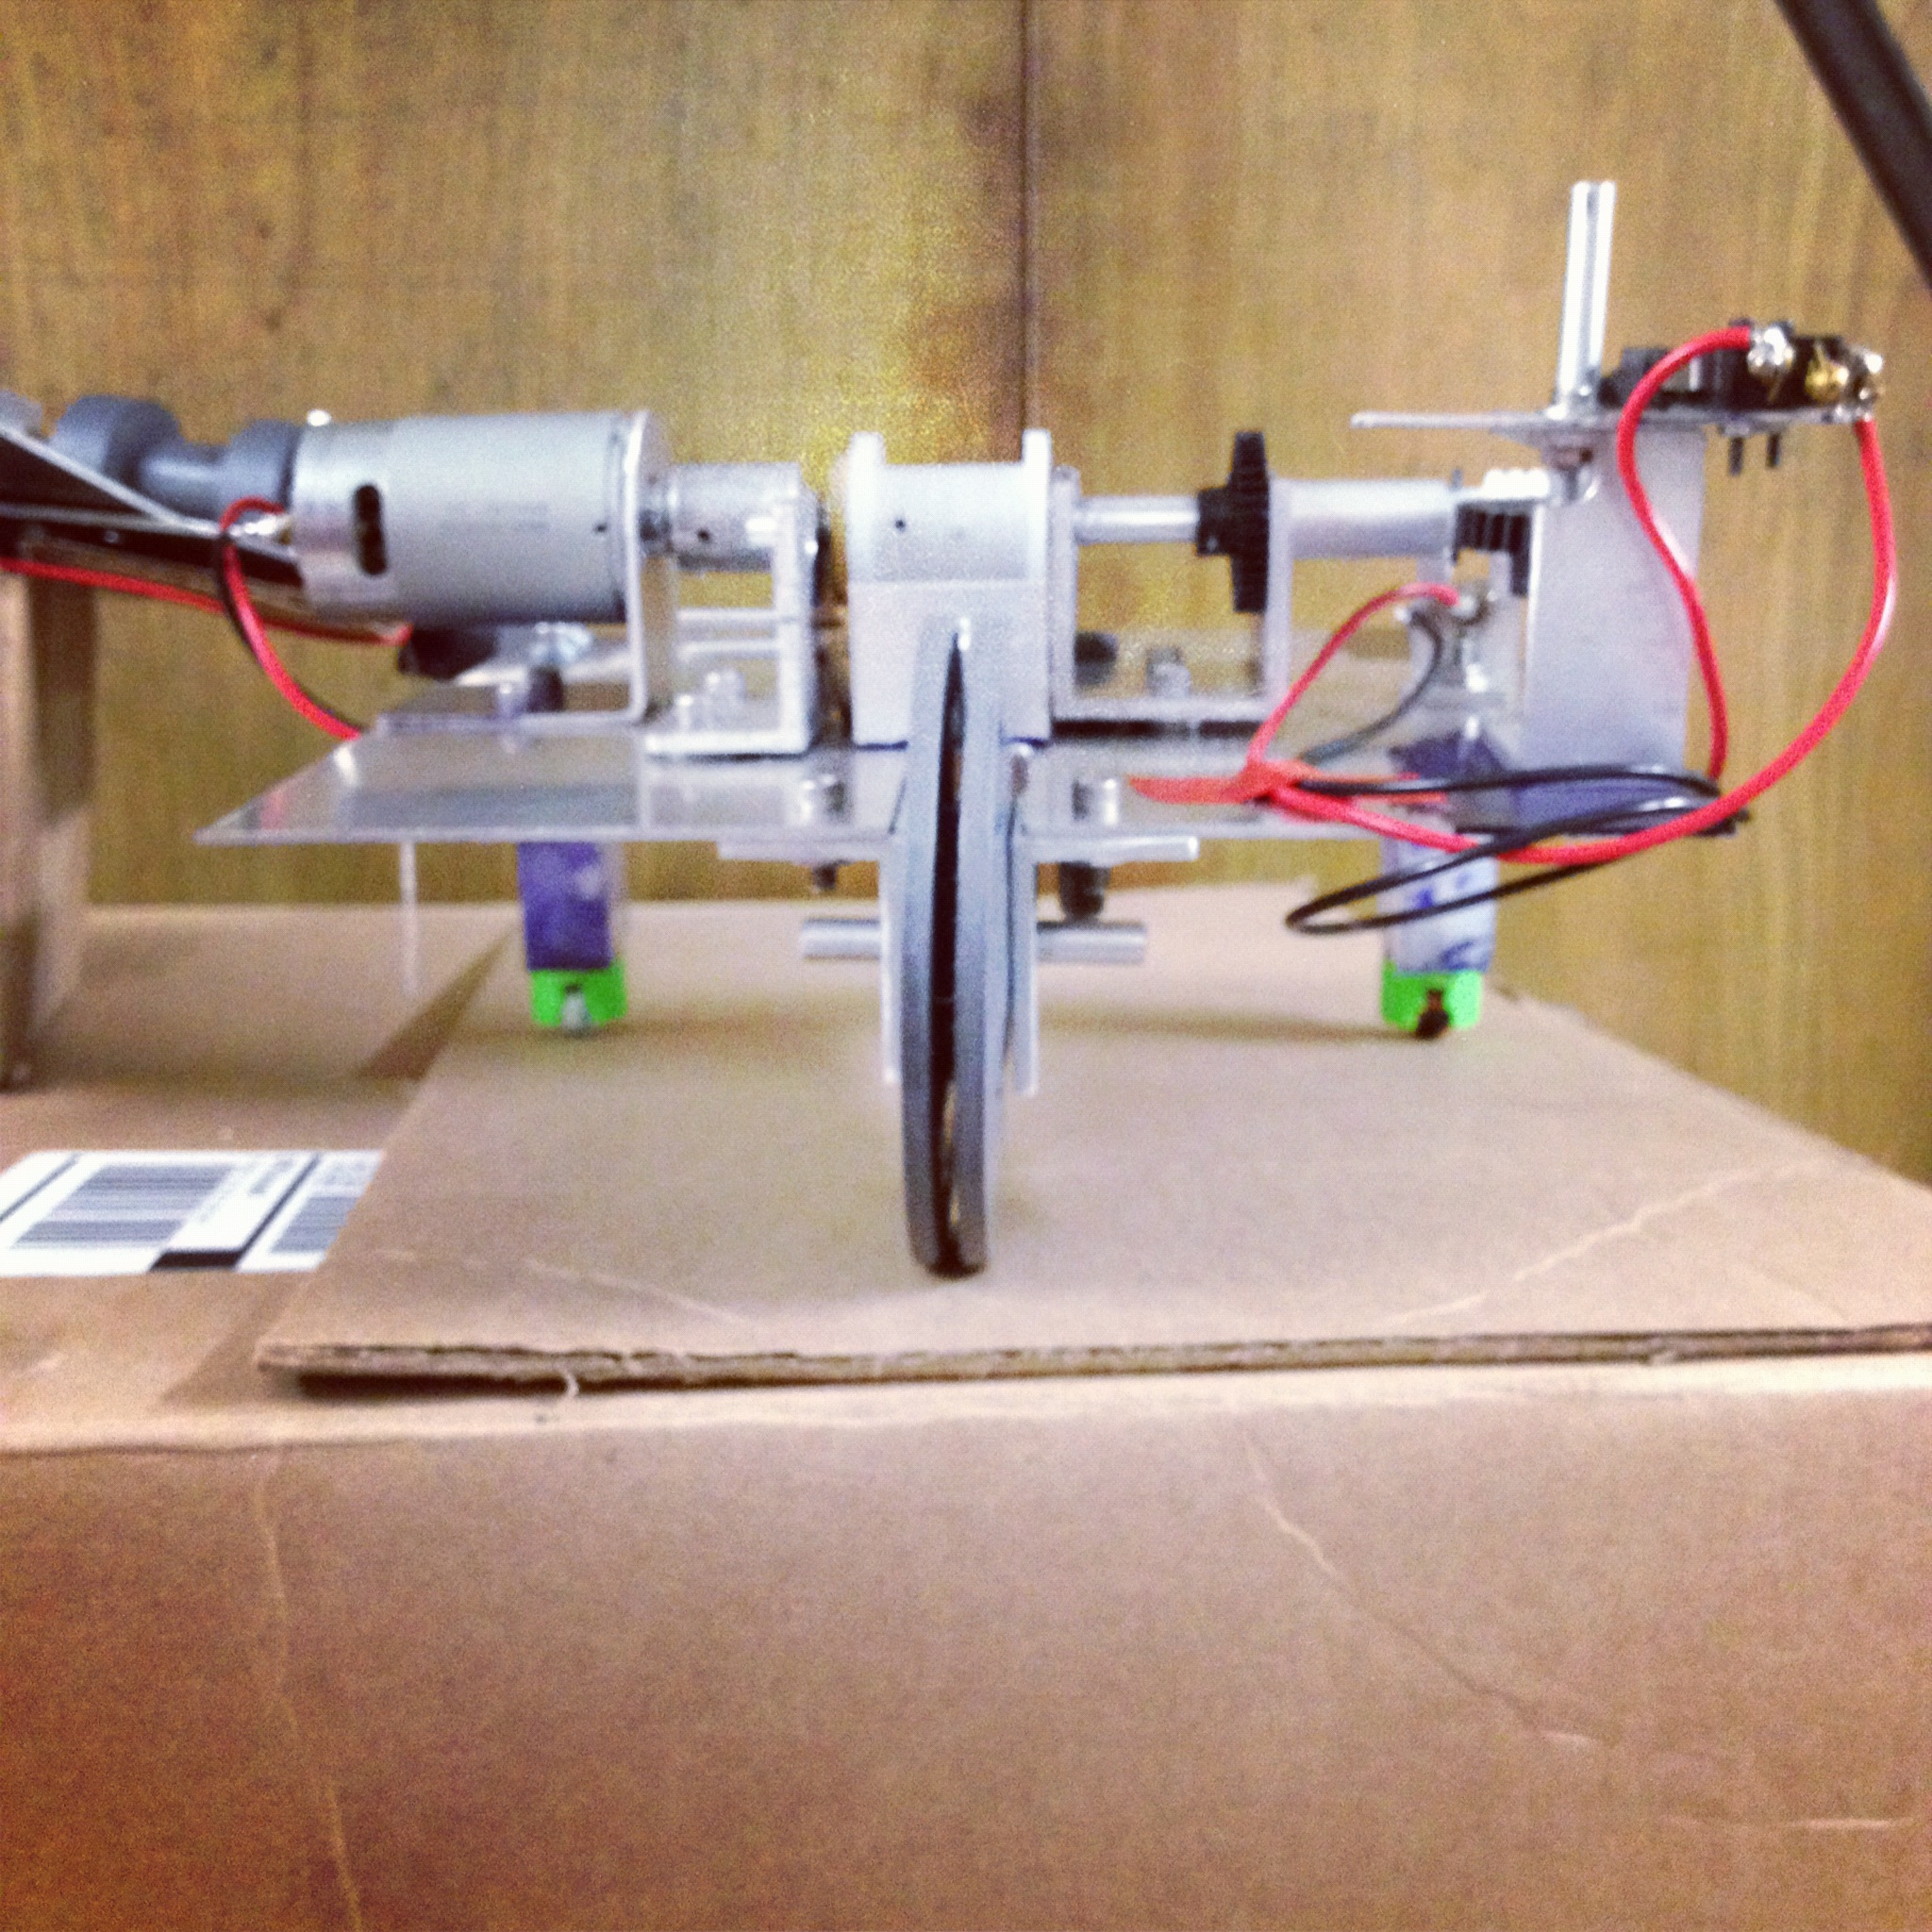
\includegraphics[height=2in, keepaspectratio]{frontview}
\end{figure}

\end{document}